\documentclass[10pt]{beamer}
\usefonttheme{professionalfonts}
\usefonttheme{serif}
\usepackage{amsmath}
\usepackage{mathtools}
%\documentclass[12pt]{beamerthemeSam.sty}
\usepackage{epsf}
%\usepackage{pstricks}
%\usepackage[orientation=portrait,size=A4]{beamerposter}
\geometry{paperwidth=160mm,paperheight=120mm}
%DT favorite definitions
\def\LL{\left\langle}	% left angle bracket
\def\RR{\right\rangle}	% right angle bracket
\def\LP{\left(}		% left parenthesis
\def\RP{\right)}	% right parenthesis
\def\LB{\left\{}	% left curly bracket
\def\RB{\right\}}	% right curly bracket
\def\PAR#1#2{ {{\partial #1}\over{\partial #2}} }
\def\PARTWO#1#2{ {{\partial^2 #1}\over{\partial #2}^2} }
\def\PARTWOMIX#1#2#3{ {{\partial^2 #1}\over{\partial #2 \partial #3}} }

\def\rightpartial{{\overrightarrow\partial}}
\def\leftpartial{{\overleftarrow\partial}}
\def\diffpartial{\buildrel\leftrightarrow\over\partial}

\def\BI{\begin{itemize}}
\def\EI{\end{itemize}}
\def\BE{\begin{displaymath}}
\def\EE{\end{displaymath}}
\def\BEA{\begin{eqnarray*}}
\def\EEA{\end{eqnarray*}}
\def\BNEA{\begin{eqnarray}}
\def\ENEA{\end{eqnarray}}
\def\EL{\nonumber\\}


\newcommand{\map}[1]{\frame{\frametitle{\textbf{Course map}}
\centerline{\includegraphics[height=0.86\paperheight]{../../map/#1.png}}}}
\newcommand{\wmap}[1]{\frame{\frametitle{\textbf{Course map}}
\centerline{\includegraphics[width=0.96\paperwidth]{../../map/#1.png}}}}

\newcommand{\etal}{{\it et al.}}
\newcommand{\gbeta}{6/g^2}
\newcommand{\la}[1]{\label{#1}}
\newcommand{\ie}{{\em i.e.\ }}
\newcommand{\eg}{{\em e.\,g.\ }}
\newcommand{\cf}{cf.\ }
\newcommand{\etc}{etc.\ }
\newcommand{\atantwo}{{\rm atan2}}
\newcommand{\Tr}{{\rm Tr}}
\newcommand{\dt}{\Delta t}
\newcommand{\op}{{\cal O}}
\newcommand{\msbar}{{\overline{\rm MS}}}
\def\chpt{\raise0.4ex\hbox{$\chi$}PT}
\def\schpt{S\raise0.4ex\hbox{$\chi$}PT}
\def\MeV{{\rm Me\!V}}
\def\GeV{{\rm Ge\!V}}

%AB: my color definitions
%\definecolor{mygarnet}{rgb}{0.445,0.184,0.215}
%\definecolor{mygold}{rgb}{0.848,0.848,0.098}
%\definecolor{myg2g}{rgb}{0.647,0.316,0.157}
\definecolor{abtitlecolor}{rgb}{0.0,0.255,0.494}
\definecolor{absecondarycolor}{rgb}{0.0,0.416,0.804}
\definecolor{abprimarycolor}{rgb}{1.0,0.686,0.0}
\definecolor{Red}           {cmyk}{0,1,1,0}
\definecolor{Grey}           {cmyk}{.7,.7,.7,0}
\definecolor{Blue}          {cmyk}{1,1,0,0}
\definecolor{Green}         {cmyk}{1,0,1,0}
\definecolor{Brown}         {cmyk}{0,0.81,1,0.60}
\definecolor{Black}         {cmyk}{0,0,0,1}

\usetheme{Madrid}


%AB: redefinition of beamer colors
%\setbeamercolor{palette tertiary}{fg=white,bg=mygarnet}
%\setbeamercolor{palette secondary}{fg=white,bg=myg2g}
%\setbeamercolor{palette primary}{fg=black,bg=mygold}
\setbeamercolor{title}{fg=abtitlecolor}
\setbeamercolor{frametitle}{fg=abtitlecolor}
\setbeamercolor{palette tertiary}{fg=white,bg=abtitlecolor}
\setbeamercolor{palette secondary}{fg=white,bg=absecondarycolor}
\setbeamercolor{palette primary}{fg=black,bg=abprimarycolor}
\setbeamercolor{structure}{fg=abtitlecolor}

\setbeamerfont{section in toc}{series=\bfseries}

%AB: remove navigation icons
\beamertemplatenavigationsymbolsempty
\title[Universal gravitation]{
  \textbf {Universal gravitation}\\
%\centerline{}
%\centering
%\vspace{-0.0in}
%\includegraphics[width=0.3\textwidth]{propvalues_0093.pdf}
%\vspace{-0.3in}\\
%\label{intrograph}
}

\author[W. Freeman] {Physics 211\\Syracuse University, Physics 211 Spring 2022\\Walter Freeman}

\date{\today}

\begin{document}

\frame{\titlepage}

\frame{\frametitle{\textbf{Announcements}}
	Help hours in the few days: (more to be added next week)
	
	\begin{itemize}
		\item Today, 9:45-10:30ish and 3:00-5:00 (Walter + coaches)
		\item {\color{Blue}Friday, 4-6 PM, room 204 (Brendan / EducationalPorpoises)}
		\begin{itemize}
			\item He is holding a workshop for people who want help learning how to ``decode'' physical situations and ``set up'' problems
		\end{itemize}
		\item Sunday, 2:30-4:30 PM, Physics Clinic or Stolkin Auditorium -- a workshop to help people prepare for Exam 2
		
	\end{itemize}
}
	

\frame{\frametitle{\textbf{A block on a ramp}}
\large
A block of mass $m_1$ rests on a ramp at angle $\theta$; a weight of mass $m_2$ hangs over the side of the ramp. The
coefficient of kinetic friction is $\mu_k$.

\bigskip

Calculate its acceleration if it:

\BI
\item{... slides down the ramp ($m_2$ is small)}
\item{... is pulled back up the ramp ($m_2$ is large)}
\EI
}


\frame{\frametitle{\textbf{An exam question from last year: a Formula 1 car}}
}

\frame{\frametitle{\textbf{The ``circular pendulum'': Otto on a string}}
}


\frame{\frametitle{\textbf{Homework questions?}}}

\frame{\frametitle{\textbf{A new force: Gravity, in general}}
  \Large
  \BI
\item{On Earth all objects experience a gravitational force proportional to their mass:}
\item{$F_{\rm{grav}} = mg$, directed down toward the Earth}
  \BI
  \large
\item{How does this work when you're not on Earth?}
\item{What determines how big $g$ is?}
  \EI
  \EI
}

\frame{\frametitle{\textbf{A brief history of gravity and the heavens}}
\large
  The history here is an interesting insight into the way scientific thought has evolved:
``How can we explain the sky?''
\BI
\item{Stars in the sky all seem to move together, but with some ``wanderers'': planets}
  \BI
\item{They appear to move in one direction, but sometimes stop and turn around}

\bigskip

\centerline{  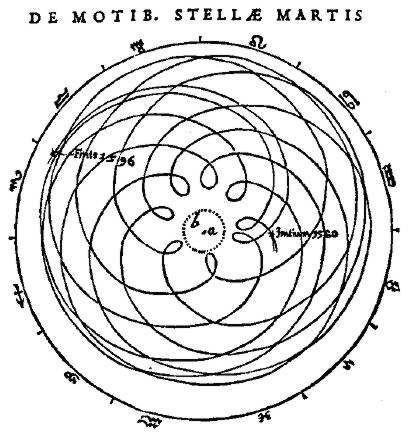
\includegraphics[width=0.3\textwidth]{Kepler_Mars_retrograde.jpg}}

  \bigskip
\item{How can we explain this?}
  \EI
  \EI
}
\frame{\frametitle{\textbf{A brief history of gravity and the heavens}}
\BI
\item{Ptolemy: Things go in circles rotating on circles, because circles are perfect, with the Earth at the center}
  \BI
\item{``Epicycles'' required to make the retrograde motion}
\EI
\item{Copernicus: Things go in circles rotating on circles, but with the Earth at the center}
  \BI
\item{Relative motion between Earth and planets responsible for retrograde motion}
  \EI
\item{Brahe: Fantastic measurements of motions of the planets (even more epicycles); geoheliocentrism}
\item{Kepler: Ellipses! No epicycles needed. Laws of planetary motion.}
\item{Galileo: Kinematics; moons of Jupiter; phases of Venus}
\item{Newton: Universal gravitation; dynamics}
  \EI
}

\frame{\frametitle{\textbf{Newtonian gravity}}
  \large
\BI
\item{All objects -- stars, planets, apples, people -- exert forces on each other}
\item{That force is given by}
\Large
  \bigskip
  
 \centerline{$F_g = \frac{GMm}{r^2}$}
\large
\bigskip
\item{Both objects feel the same force, directed toward each other}
\item{Note:}

  \bigskip
\Large
    \centerline{$a_g = F_g/m = \frac{GM}{r^2}$}
\large
    \bigskip

  \item{What is $G$?}
\item{$\rightarrow$ \color{Red} Fundamental constant of nature that tells us how strong gravity is}
\EI
}

\frame{

\Large

What are the units of $G$? 

\bigskip

(Remember, it appears in the equation $F_g = \frac{GMm}{r^2}$)

\BI

\item{a) $\rm m/\rm s^2$}
\item{b) $\rm m^2/\rm s^2$}
\item{c) $\rm N \cdot m^2/\rm kg^2$}
\item{d) $\rm m^3 \rm kg^{-1} \rm s^{-2}$}

\EI
}

\frame{\frametitle{\textbf{Newtonian gravity}}
  \large
\BI
\item{All objects -- stars, planets, apples, people -- exert forces on each other}
\item{That force is given by}

  \bigskip
  
 \centerline{$F_g = \frac{GMm}{r^2}$}

\bigskip
\item{Both objects feel the same force, directed toward each other}
\item{Note:}

  \bigskip

    \centerline{$a_g = F_g/m = \frac{GM}{r^2}$}

    \bigskip

  \item{What is $G$?}
  \BI
\item{Fundamental constant of nature that tells us how strong gravity is}

  \bigskip

  \centerline{  \Large$G=6.673\times10^{-11} \frac{\rm N\cdot\rm m^2}{\rm{kg}^2}$}

\bigskip

\item{This is really, really tiny}
  \EI
  \EI
}

\frame{\frametitle{\textbf{Measuring $G$}}
  \centerline{  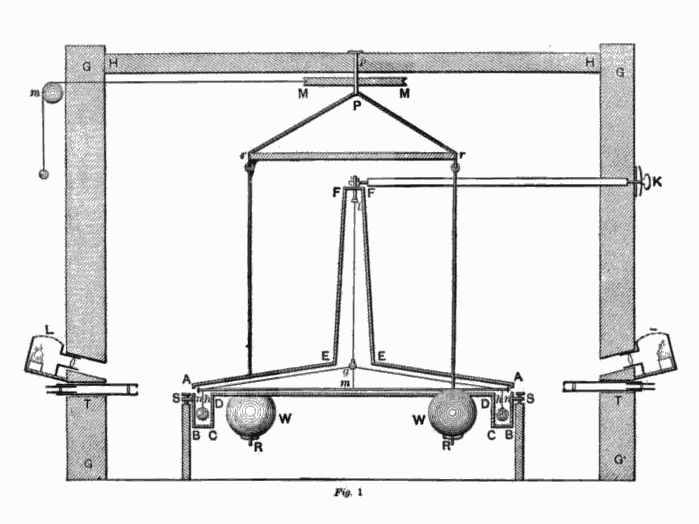
\includegraphics[width=0.8\textwidth]{Cavendish_Experiment.png}}

  \pause

  \centerline{\Large What is the force between a 1kg mass and a 5kg mass that are 5cm apart?}

\large

}
\frame{\frametitle{\textbf{Measuring $G$}}
  \centerline{  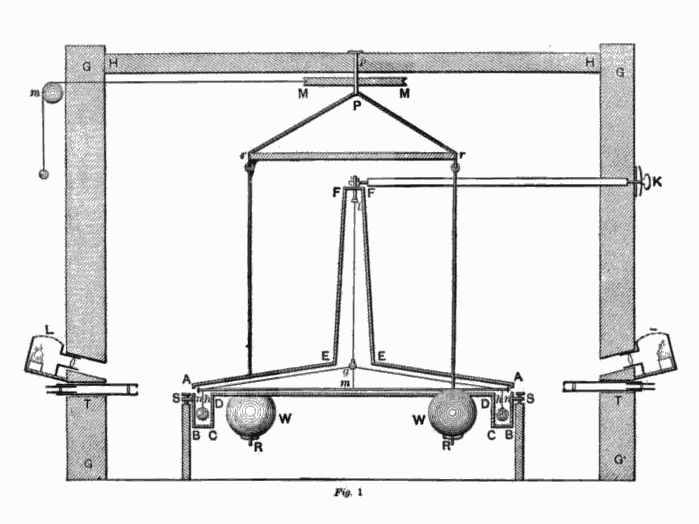
\includegraphics[width=0.4\textwidth]{Cavendish_Experiment.png}}


  \centerline{\Large What is the force between a 1kg mass and a 5kg mass that are 5cm apart?}

\large


\bigskip
\bigskip
\bigskip
\bigskip
\begin{center}
Back of the envelope math (in SI units): 

$F_g \approx \frac{(7 \times 10^{-11})(5)(1)}{5 \times 10^{-2}} = 7 \times 10^{-9}$ N!
\end{center}
}


\frame{\frametitle{\textbf{Measuring the mass of the Earth}}

  \Large \centerline{  What is the mass of the Earth?}

  \pause

We have two expressions for the gravitational force:

\BI
\item{$F_g = mg$, where $g$ is an empirical measurement of Earth's gravity}
\item{$F_g = GMm/r^2$, giving the force between any two objects (not just on Earth}
\EI

\bigskip

  $F_g = \frac{GMm}{r^2} = mg$


  \bigskip

  \pause

  $M = \frac{gR^2}{G} = 5.97 \times 10^{24}$ kg...
}

\frame{\frametitle{\textbf{Gravity and circular motion}}
  \Large
  \begin{itemize}
    \item{Many orbits are nearly circular}
    \item{Everything you learned on Tuesday about uniform circular motion still applies}
    \item{Weighing the Earth by looking at the Moon:}
      \BI
      \Large
    \item{$F_g = \frac{GM_e M_m}{r^2} = M_m \omega^2 r$}
      \EI
    \item{These problems are nothing new and nothing hard; it's just a new force}
    \item{Problems involving orbits are often easier (fewer forces)}
      \EI
}
\end{document}



